\section{A method for flexible performance-complexity balancing}\label{sec:our-method}

Our work builds on the HARP method \cite{chen_harp_2018} for pretraining methods such as node2vec \cite{grover_node2vec_2016} on coarsened graphs. The sequence \( G_0, G_1, G_2, \dots, G_L \) is generated in HARP consecutively. In an overview, the HARP algorithm first ahead-of-time consecutively coarsens the graph. The method itself can then be executed by repeating the following steps on the graphs from the coarsest to the finest (i.e., from \( G_L \) to \( G_0 \)):
\begin{enumerate}
  \item \textbf{Training on an intermediary graph}. The graph embedding model is trained on \( G_i \), producing its embedding \( \Phi_{G_i} \).
  \item \textbf{Embedding prolongation}. The embedding \( \Phi_{G_i} \) is \textit{prolonged} into \( \Phi_{G_{i - 1}} \) by copying embeddings of merged nodes. \( \Phi_{G_{i - 1}} \) is then used as the starting point for training on \( G_{i - 1} \).
\end{enumerate}

While the prolongation used by HARP is sufficient when used as a means of pre-training, the approach is far too crude when studying the relationship between graph complexity and the quality of graph embedding. In order to overcome this limitation, we present the adaptive prolongation approach. This algorithm works with the pre-coarsened graphs produced by HARP, however, the embedding is learned in a different manner. There are \( K \) prolongation steps (where generally \( K \neq L \)) and each of them uses all graphs \( G_L, \dots, G_0 \). The prolongation steps are driven by local properties of the graph with relation to the downstream task, allowing for different levels of granularity in different parts of the graph. Let us denote \( \Psi_K, \dots, \Psi_0 \) the resulting embedding sequence. The algorithm starts with the coarsest graph \( G_L \), trains a graph model to compute its embedding \( \Psi_K \) and gradually refines it until reaching the embedding \( \Psi_0 \). These prolongation steps are interlaid with continued training of the graph model, as in standard HARP. A description of a single prolongation step from \( \Psi_{i + 1} \) to \( \Psi_i \) is schematically outlined in Figure~\ref{fig:adaptive-prolongation} and described in detail in Appendix \ref{sec:app:prolongation-step}.

\begin{figure}
  \centering
  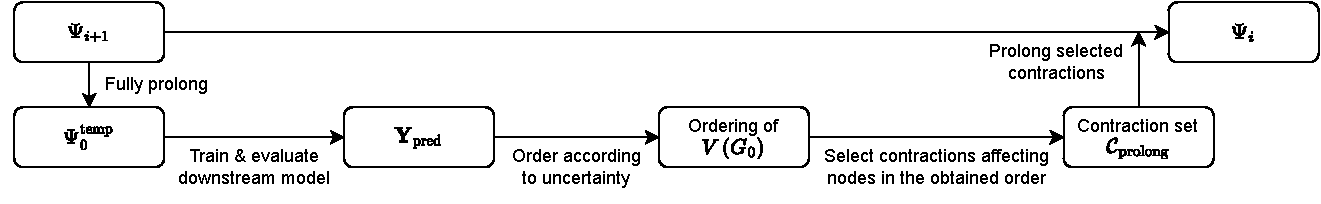
\includegraphics[width=0.9\textwidth]{images/adaptive-prolongation/adaptive-prolongation.pdf}
  \caption{A schematic explanation of the adaptive prolongation algorithm for obtaining the embedding \( \Psi_{i} \) from \( \Psi_{i + 1} \).}
  \label{fig:adaptive-prolongation}
\end{figure}
